\documentclass[25pt, a0paper, landscape]{tikzposter}
\tikzposterlatexaffectionproofoff

% Preamble
\usepackage{tikz}
\usetikzlibrary{positioning}
\usetikzlibrary{arrows.meta,arrows}
\usepackage{tcolorbox}
\usepackage{xcolor}
\usepackage[backend=biber,doi=false,url=false,isbn=false,eprint=false]{biblatex}
\usepackage{colortbl}
\usepackage[default,oldstyle,scale=0.95]{opensans} %% Alternatively
%% use the option 'defaultsans' instead of 'default' to replace the
%% sans serif font only.
\usepackage[T1]{fontenc}
\usepackage{tikz,pgfplots,pgfplotstable}
\pgfplotsset{compat=1.8}
\usepackage{enumitem}
\usepackage{titlesec}
\usepackage{graphicx}

% Layout
\renewcommand*{\bibfont}{\footnotesize}
\titlespacing*{\subsection}{0pt}{.5\baselineskip}{.5\baselineskip}
\definecolor{GeoDataViz_blue}{HTML}{009ADE}
\definecolor{GeoDataViz_magenta}{HTML}{FF1F5B}
\definecolor{GeoDataViz_green}{HTML}{00cd6c}

\definecolor{GeoDataViz_purple}{HTML}{AF58BA}
\definecolor{GeoDataViz_yellow}{HTML}{FFC61E}
\definecolor{GeoDataViz_orange}{HTML}{F28522}

\definecolor{GeoDataViz_amber}{HTML}{FFAA00}
\definecolor{GeoDataViz_red}{HTML}{E9002D}

\definecolor{BlockColor}{HTML}{9c64e0}

\newcommand*\circled[1]{\tikz[baseline=(char.base)]{%
		\node[shape=circle,fill=white,text width=1em,align=center,draw=none,text=BlockColor,inner sep=2pt] (char) {#1};}}

%% Title
\colorlet{backgroundcolor}{white}
\definetitlestyle{mytitle}{
	width=.992\textwidth,
	titletoblockverticalspace=0pt,
}{\begin{scope}[line width=\titlelinewidth,]
	\end{scope}}

\usetitlestyle{mytitle}
%% Title wrap
\makeatletter
\def\title#1{\gdef\@title{\scalebox{\TP@titletextscale}{%
			\begin{minipage}[t]{\linewidth}
				#1
				\par
			\end{minipage}%
		}}}
\makeatother
%% Title structure
\makeatletter
\renewcommand\TP@maketitle{%
	\begin{minipage}[t]{0.35\linewidth}
		\color{titlefgcolor}
		{\fontseries{sb}\selectfont \Huge {\@title}}
		{\large \@author \par}
		{\@institute \par}
	\end{minipage}%
	\hfill
	\begin{minipage}[t]{0.65\linewidth}
		~\\
		\hspace*{\fill}\@titlegraphic
	\end{minipage}
}
\makeatother

% Block
\defineblockstyle{myblock}{
	titleleft, roundedcorners=0, linewidth=10pt
}{
	\draw[color=framecolor, fill=blockbodybgcolor,
		rounded corners=\blockroundedcorners] (blockbody.south west)
	rectangle (blockbody.north east);
	\ifBlockHasTitle
		\draw[color=framecolor, fill=blocktitlebgcolor,
			rounded corners=\blockroundedcorners] (blocktitle.south west)
		rectangle (blocktitle.north east);
	\fi
}
\useblockstyle{myblock}
%% Block height

\newcommand{\myemph}[1]{{\fontseries{sb}\selectfont\color{black} #1}}


% Metadata
\title{Classifier-based latency estimation for covert attention ERP decoding}
\author{
	Arne Van Den Kerchove\textsuperscript{*,1,2},
	Hakim Si-Mohammed\textsuperscript{1},
	Marc Van Hulle\textsuperscript{2},
	François Cabestaing\textsuperscript{1}
}
\date{\today}
\institute{
	\textsuperscript{1}UMR CRIStAL, Univ. de Lille, Lille, France \\
	\textsuperscript{2}Lab for Neuro- and Psychophysiology, KU Leuven, Leuven, Belgium}
\titlegraphic{
	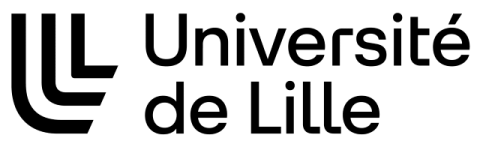
\includegraphics[height=8em]{figures/ulille.png}\hspace{1em}
	
\includegraphics[height=8em]{figures/cristal.png}\hspace{1em}
	
\includegraphics[height=8em]{figures/kul.png}
}
\addbibresource{references.bib}

\begin{document}
\maketitle
\begin{columns}
	\column{0.33333333333333333333333}
	\colorlet{blockbodybgcolor}{black!10}
	\colorlet{blockbodyfgcolor}{black!80}
	\colorlet{blocktitlebgcolor}{BlockColor}
	\colorlet{blocktitlefgcolor}{white}
	\colorlet{framecolor}{black!50}
	\block{\circled{1} Gaze-independent visual oddball interface}{
		\subsection*{\color{black} Eye motor disability}

		\begin{minipage}{.5\linewidth}
			The BCI target population suffers from eye motor disabilities, warranting the development of gaze-independent communication paradigms.
			While other active BCI modalities (auditory, somatosensory, ...) can work, visual paradigms exploiting spatial attention often yield the highest ITR~\cite{Riccio2012}.
			We aim to design a visual oddball interface that can be operated efficiently by gaze-impaired patients through accurate covert attention classification.
		\end{minipage}%
		\hfill
		\begin{minipage}{.46\linewidth}

			\centering
			\textcolor{black}{Eye motor disability incidence \\ in patient populations (\%)}
			\bigskip


			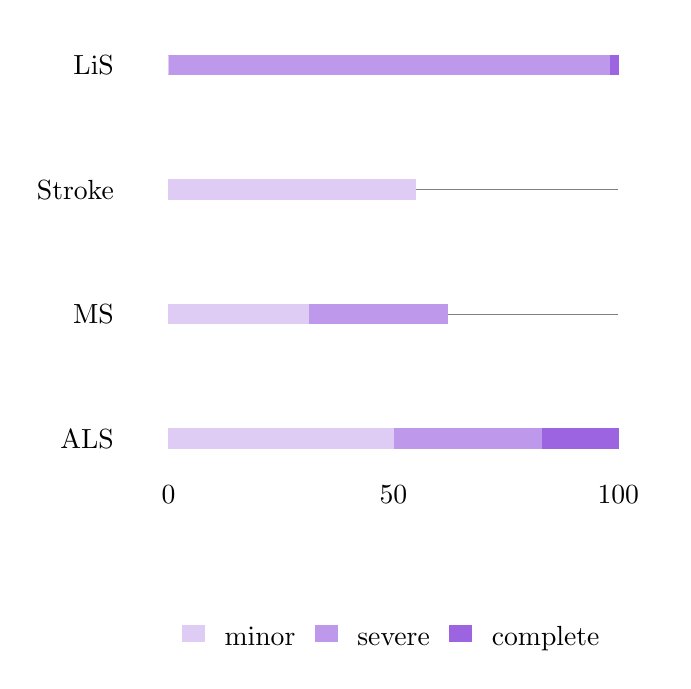
\begin{tikzpicture}
				\begin{axis}[
						xbar stacked,
						symbolic y coords ={ALS,MS,Stroke,LiS},
						yticklabels={ALS,MS,Stroke,LiS},
						ytick={ALS,MS,Stroke,LiS},
						%xlabel={incidence},
						bar width=.7em,
						legend style={
								at={(0.5,-0.30)},
								anchor=north,
								legend columns=-1,
								draw=none,
								fill=none,
								column sep=.5em,
							},
						axis line style={draw=none},
						tick style={draw=none},
						xtick={0, 50, 100}
					]
					\addplot+[fill=BlockColor!33, draw=BlockColor!33] coordinates{
							(50,ALS)
							(31,MS)
							(55,Stroke)
							(0,LiS)
						};
					\addplot+[fill=BlockColor!66, draw=BlockColor!66] coordinates{
							(33,ALS)
							(31,MS)
							(0,Stroke)
							(98,LiS)
						};
					\addplot+[fill=BlockColor, draw=BlockColor] coordinates{
							(17,ALS)
							(0,MS)
							(0,Stroke)
							(2,LiS)
						};

					\legend{\strut minor, \strut severe, \strut complete}
					\draw[color=gray] (axis cs:0,LiS) to (axis cs:100,LiS);
					\draw[color=gray] (axis cs:0,Stroke) to (axis cs:100,Stroke);
					\draw[color=gray] (axis cs:0,MS) to (axis cs:100,MS);
					\draw[color=gray] (axis cs:0,ALS) to (axis cs:100,ALS);

				\end{axis}




			\end{tikzpicture}

			%\begin{tabular}{@{}|l|rrr|r|@{}}
			%	\hline
			%	         & ALS  & MS   & Stroke  &
			%	\cellcolor{BlockColor}\textbf{LiS}                                         \\ \hline
			%	Minor    & 50\% & 31\% & 40-70\% & \cellcolor{BlockColor}                  \\
			%	Severe   & 33\% & 3\%  & +       & \cellcolor{BlockColor}\color{black}98\% \\
			%	Complete & 17\% & -    & +       & \cellcolor{ALignment improves SNR}\color{black}2\%  \\ \hline
			%\end{tabular}
		\end{minipage}


		\subsection*{\color{black} Conventional visual attention settings}
		%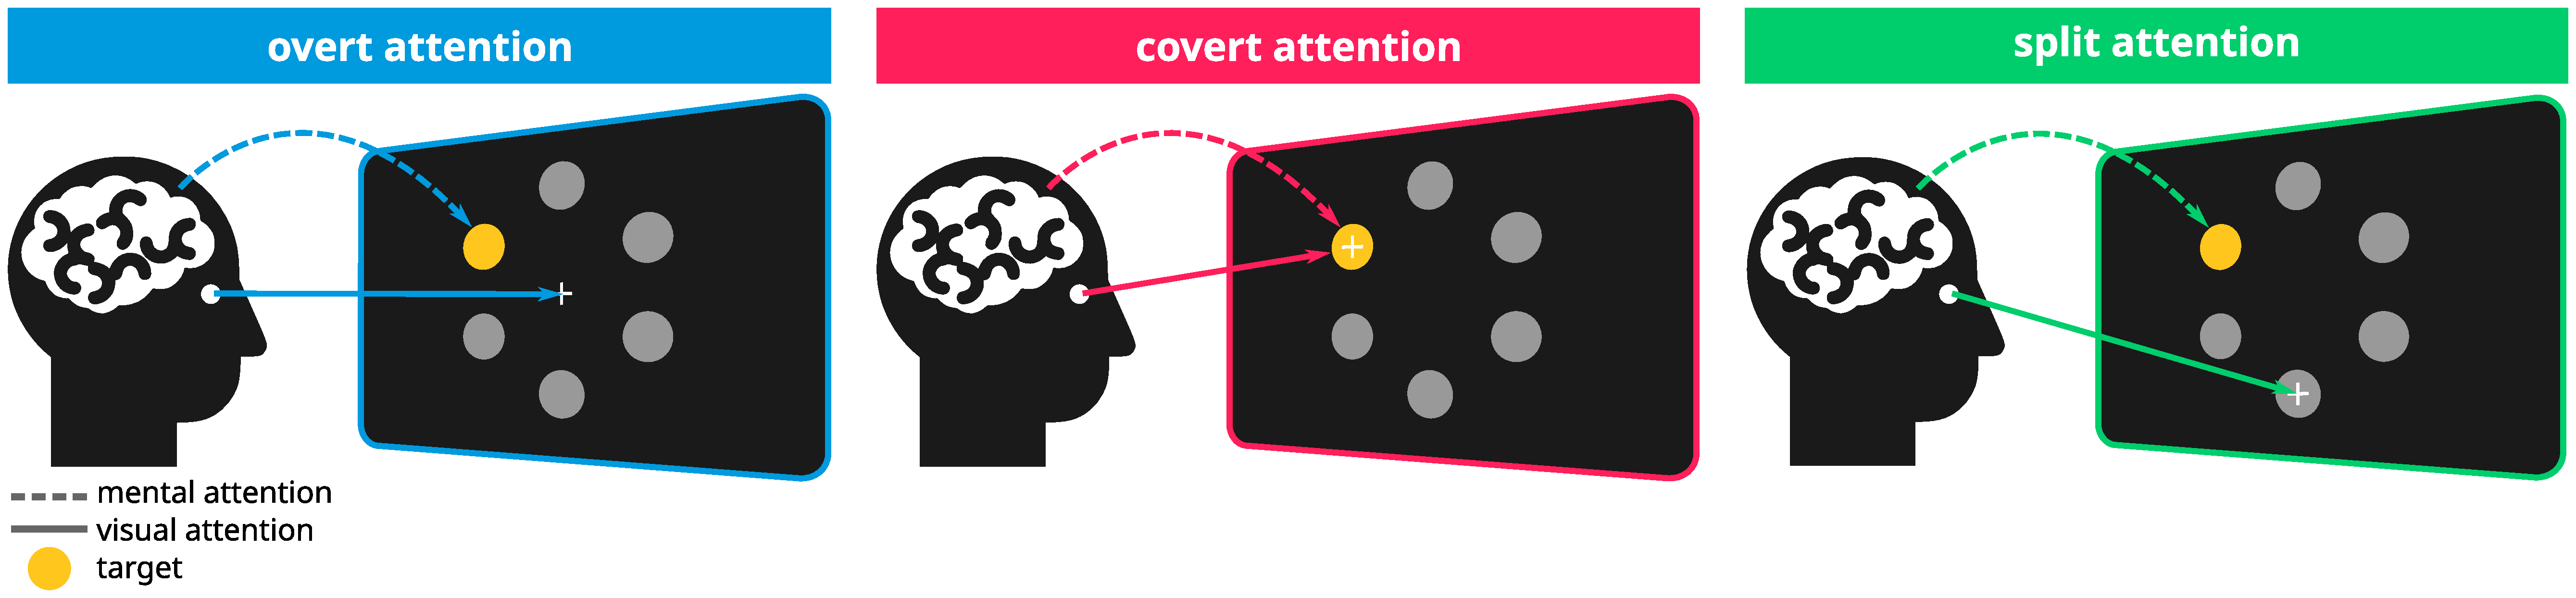
\includegraphics[width=\linewidth]{figures/attention_modes.eps}
		%Usually, a visual brain-computer interface is operated in \textbf{overt} attention mode, where the user directs their gaze to the intended target.
		%Patients with eye motor disabilities are not always able to comfortably perform overt attention.
		%Hence, \textbf{covert} attention paradigms have been designed where the user gazes at the center of the screen and selects targets in their visual periphery. Covert attention suffers from poor decoding performance, but this can be improved using \textbf{jitter correction}~\cite{Arico2014}. Further dissociating mental and visual attention

		%		\note{overt attention}

		\begin{minipage}{.48\linewidth}
			\centering
			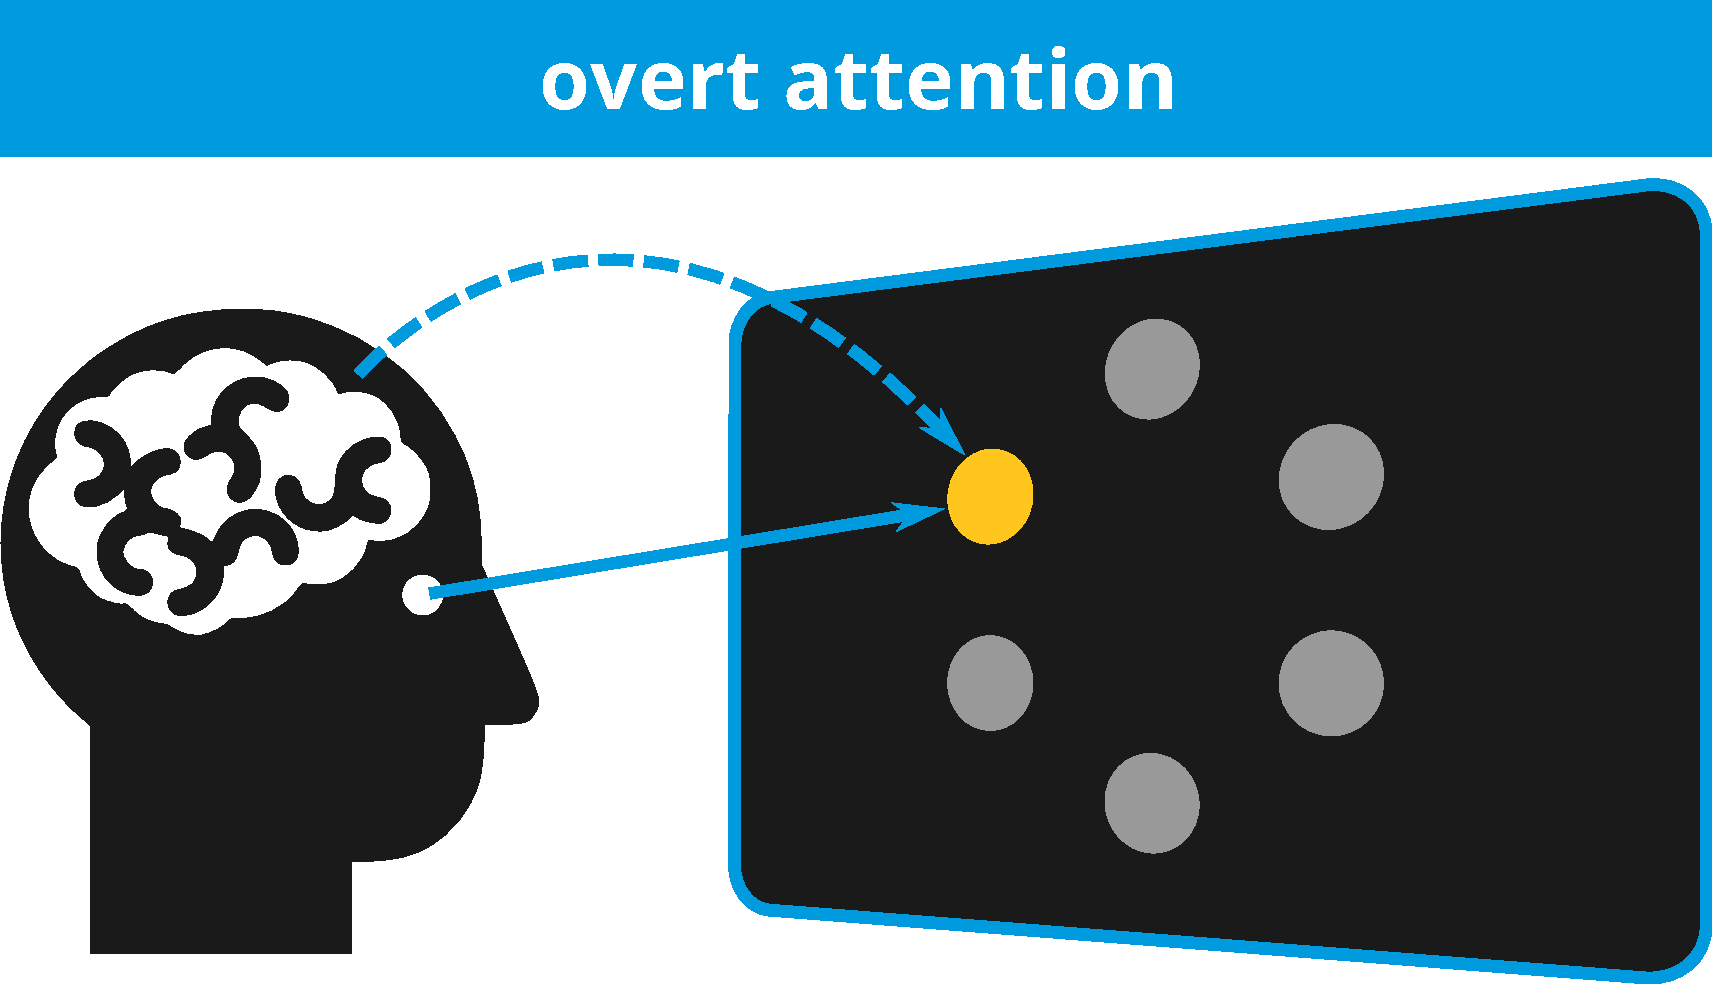
\includegraphics[width=.8\linewidth]{figures/attention_overt.pdf}
		\end{minipage}%
		\hfill%
		\begin{minipage}{.48\linewidth}
			\begin{tcolorbox}[sharp corners=all,
					colback=GeoDataViz_blue,coltext=white,
					fontupper=\bfseries,boxrule=0mm,boxsep=5mm,
				]
				Overt attention
			\end{tcolorbox}

			Persons with full eye motor control can gaze at intended targets.
		\end{minipage}%
		\bigskip
		\bigskip


		\begin{minipage}{.48\linewidth}
			\centering
			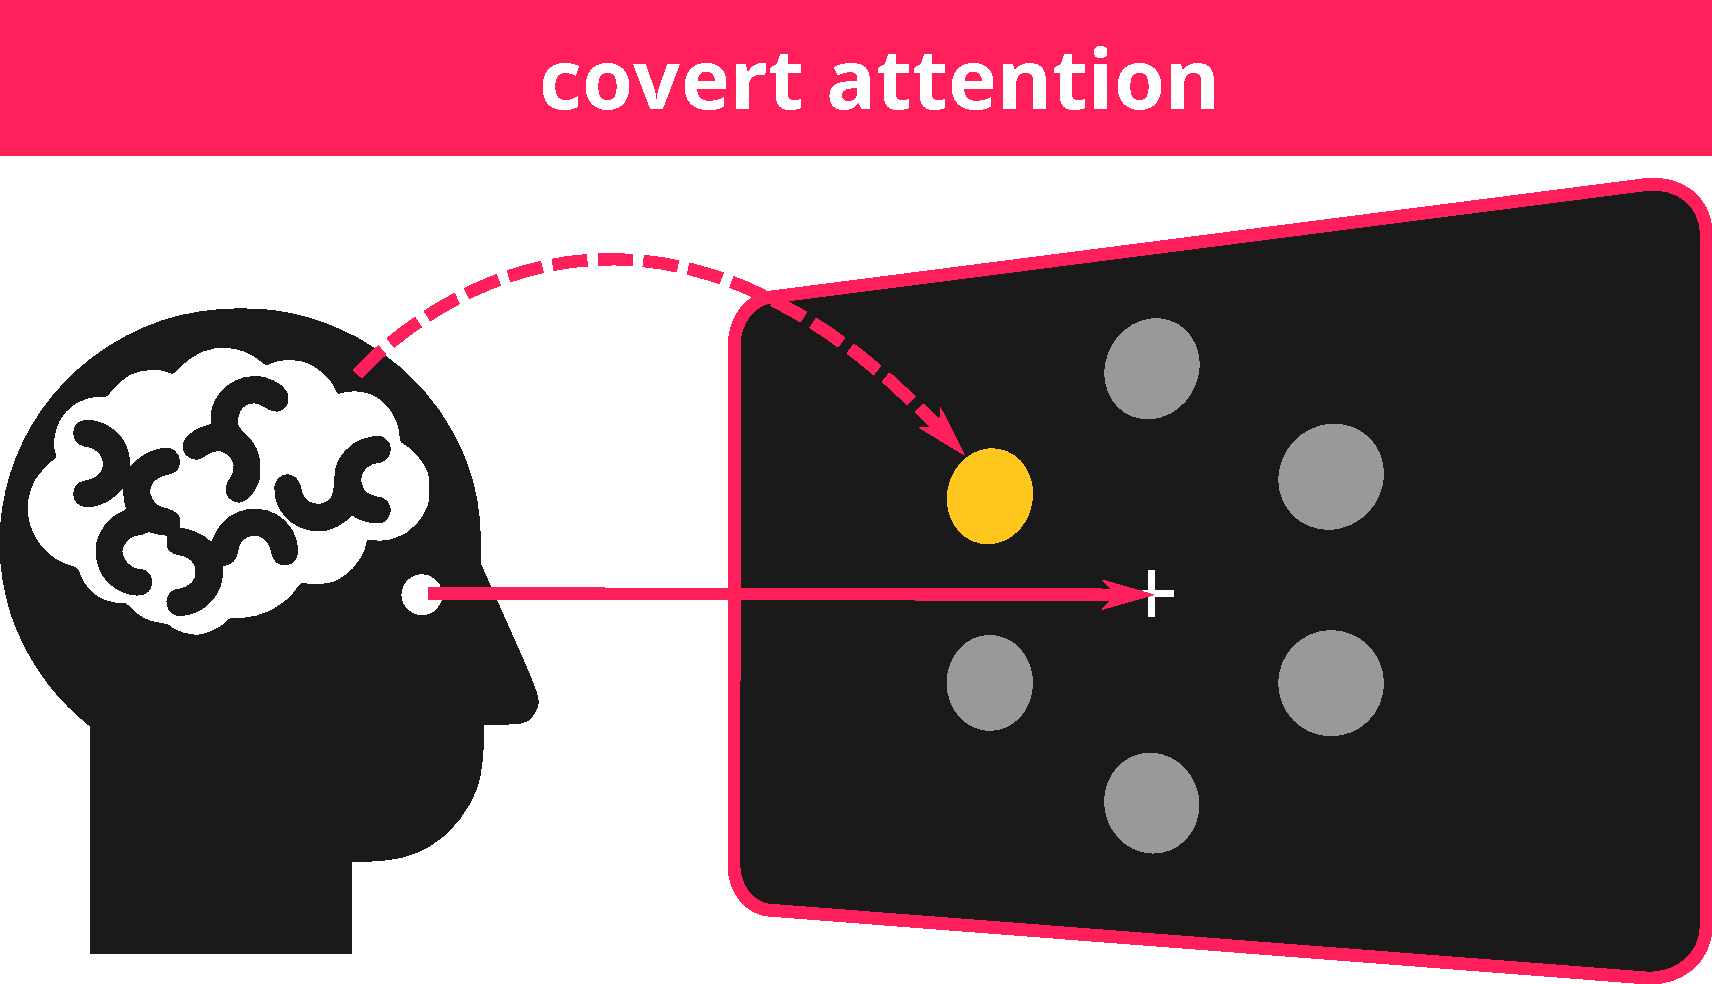
\includegraphics[width=.8\linewidth]{figures/attention_covert.pdf}
		\end{minipage}%
		\hfill%
		\begin{minipage}{.48\linewidth}
			\begin{tcolorbox}[sharp corners=all,
					colback=GeoDataViz_magenta,coltext=white,
					fontupper=\bfseries,boxrule=0mm,boxsep=5mm,
				]
				Covert attention
			\end{tcolorbox}

			Fixating the gaze at the center is a common solution, but this also requires a degree of eye motor control.
		\end{minipage}%
		\bigskip
		\bigskip

		\subsection*{\color{black} Proposed visual attention setting}


		\begin{minipage}{.48\linewidth}
			\centering
			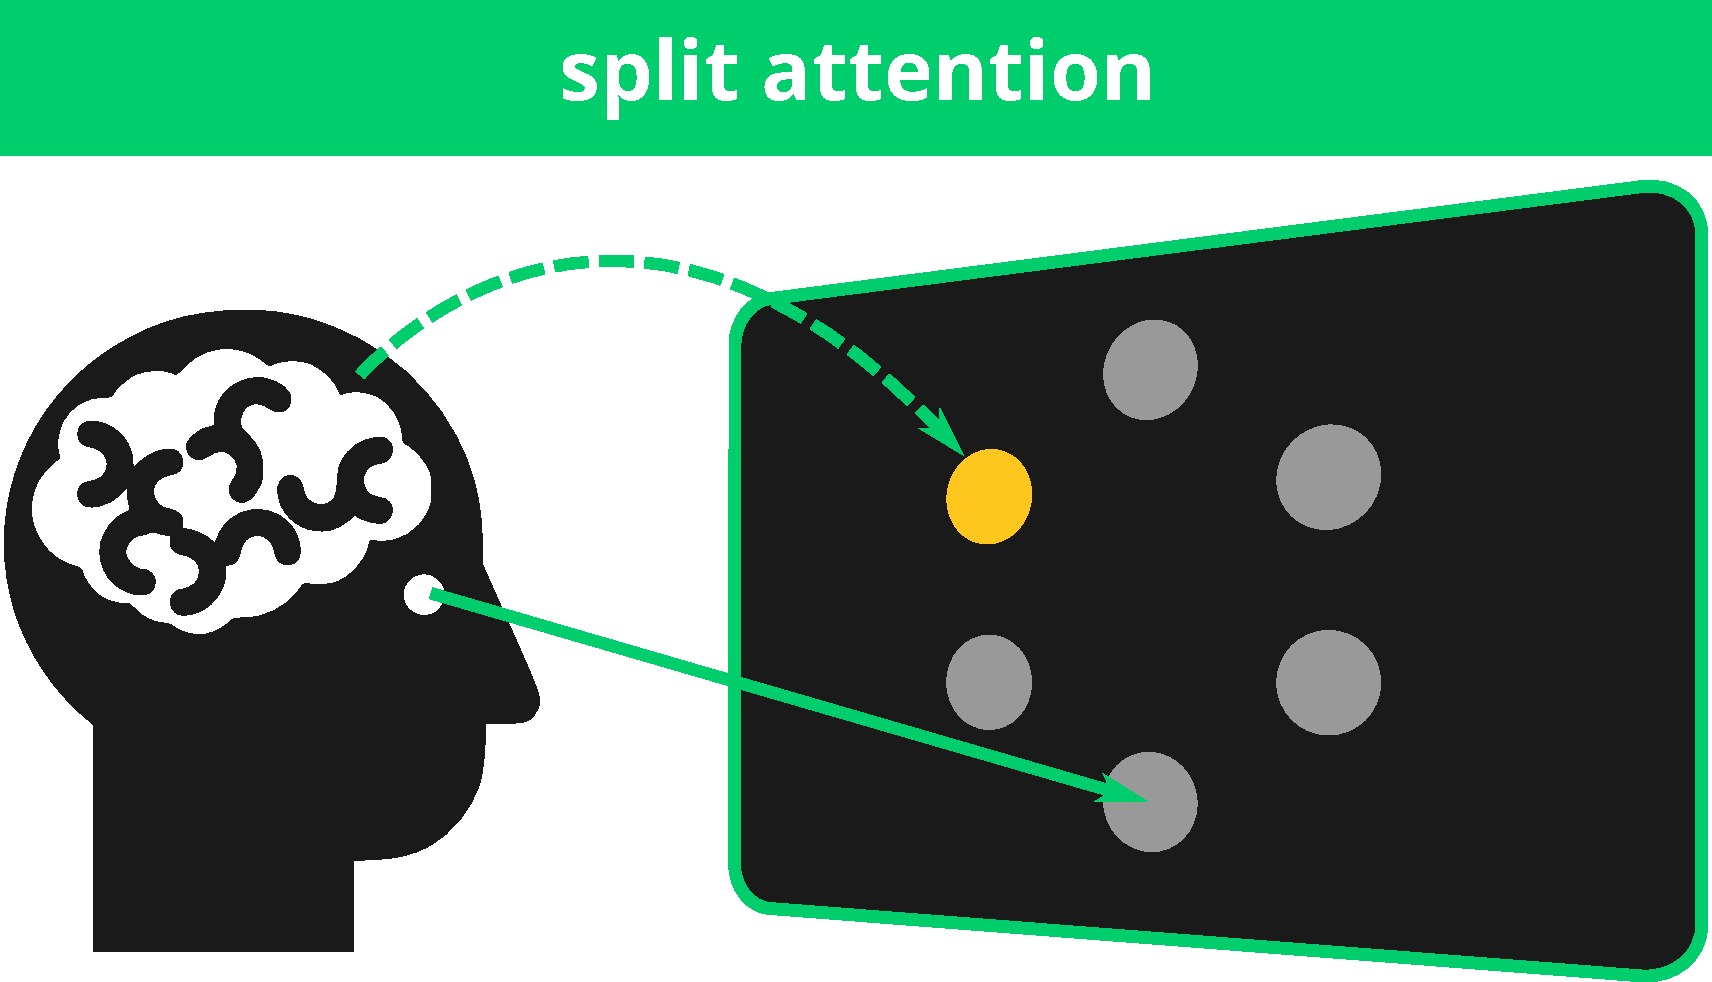
\includegraphics[width=.8\linewidth]{figures/attention_split.pdf}
		\end{minipage}%
		\hfill%
		\begin{minipage}{.48\linewidth}
			\begin{tcolorbox}[sharp corners=all,
					colback=GeoDataViz_green,coltext=white,
					fontupper=\bfseries,boxrule=0mm,boxsep=5mm,
				]
				Split attention
			\end{tcolorbox}

			We design an interface that allows for the split attention conditions that can occurr in patients with involuntary eye movements.
		\end{minipage}%




		\subsection*{\color{black} Experimental protocol}

		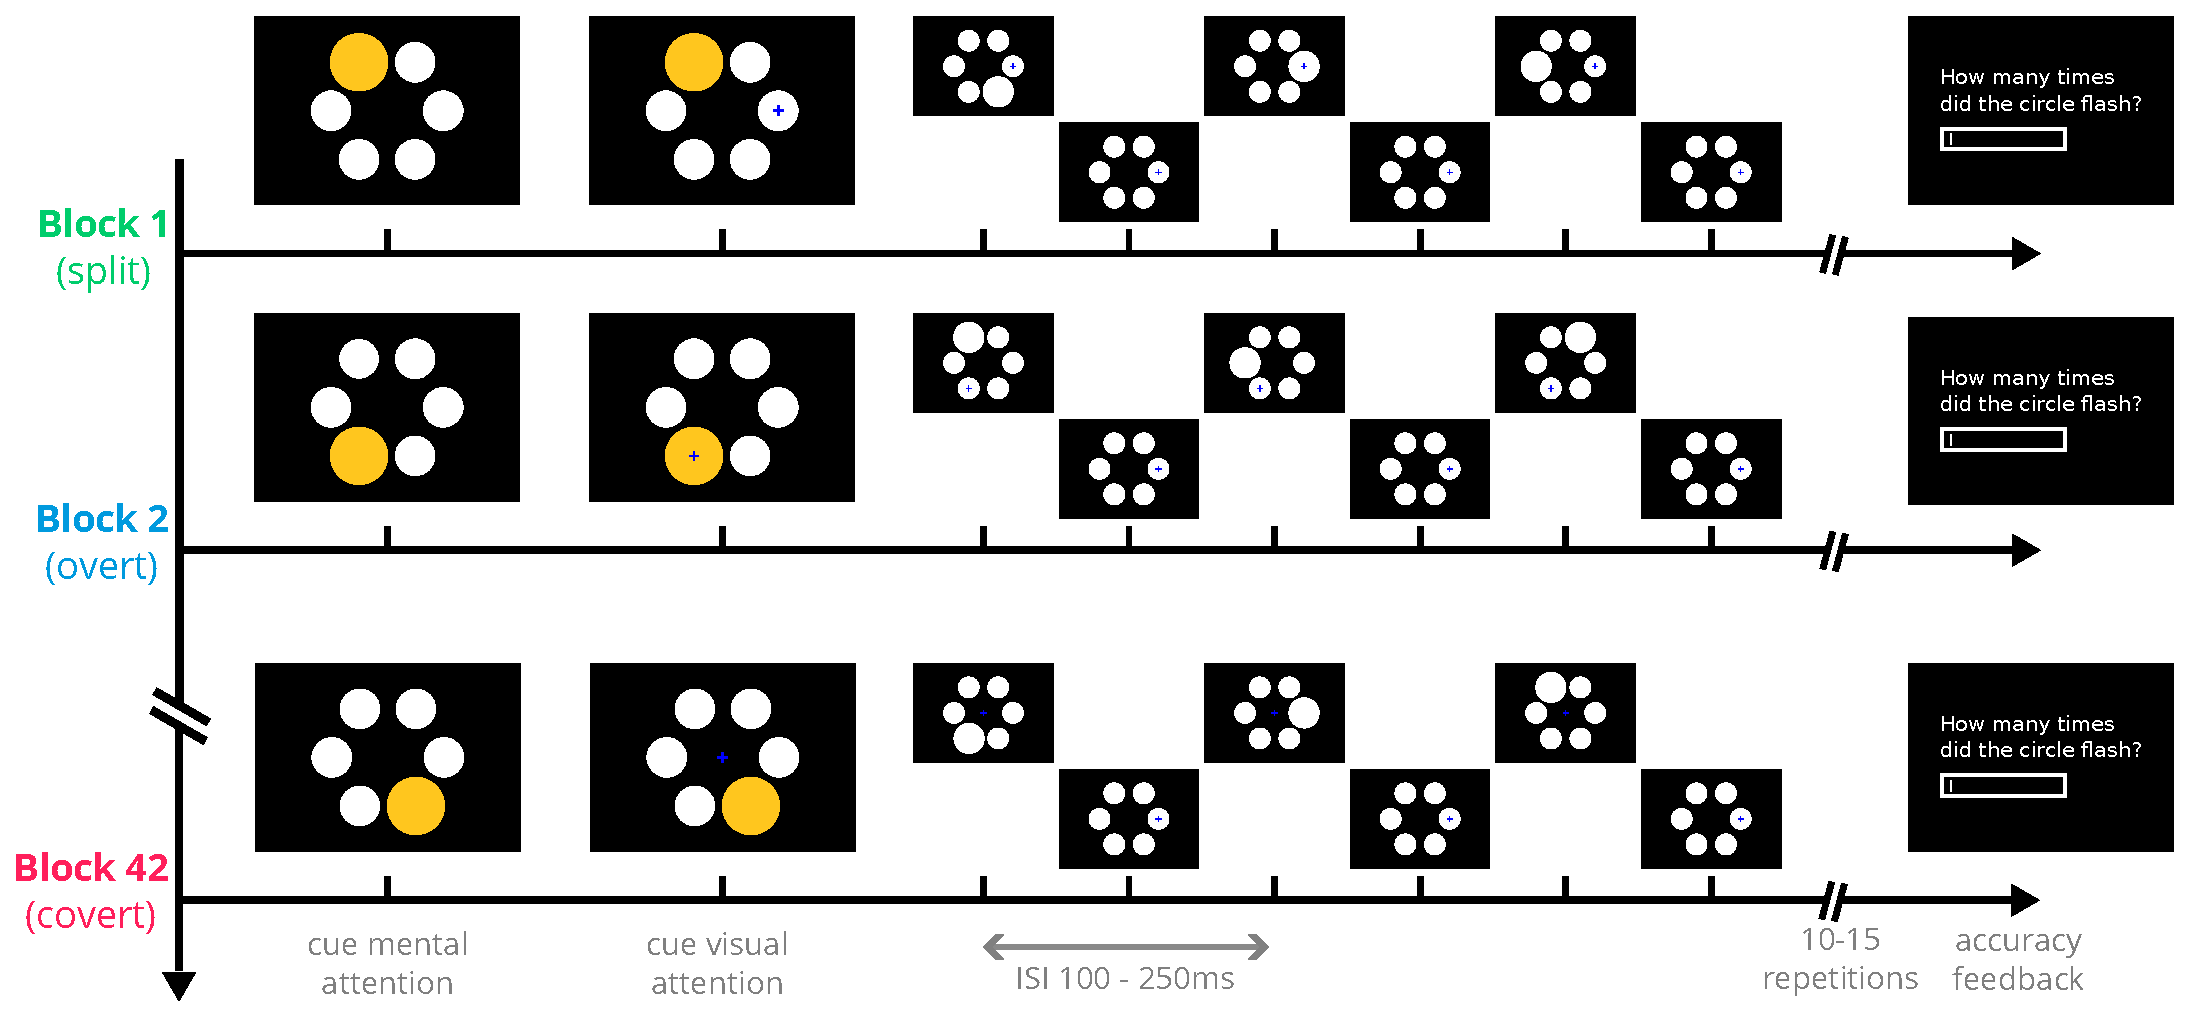
\includegraphics[width=\linewidth]{figures/timeline.eps}
	}


	\column{0.333333333333333333333333333333333333333333}
	\block{\circled{2} Novel ERP latency estimation procedure}{
		\subsection*{\color{black} The jitter problem}
		Latency jitter correction improves covert attention decoding performance~\cite{Arico2014}.
		High jitter decreases SNR when averaging over multiple trials.
		In order to correct for jitter, an algorithm must accurately estimate single-trial ERP latencies.
		Classifier-based latency estimation~\cite{Mowla2017}, paired with a time-regularized linear classifier~\cite{Sosulski2022} is a technique that can be used classify jittered signals and extract latencies.
		We propose a more accurate latency estimation and classification algorithm that iteratively applies classifier-based latency estimation.


		\subsection*{\color{black} Woody Classifier-Based Latency Estimation (wCBLE)}
		\begin{tikzfigure}
			\begin{tikzpicture}[
					line width=2pt
				]
				\node[draw,align=center](class){Spatiotemporal \\ classifier weights};
				\node[below=of class,align=center](xcorr) {cross-correlation};
				\node[draw, below=of xcorr,align=center](score) {score over time};
				\node[below=.5of score](a1){};
				\node[draw,below=.5 of a1,align=center, xshift=-1.5in](latency) {Latencies};
				\node[draw,below=.5 of a1,align=center,xshift=1.5in](wav) {Wavelet coefs};
				\node[draw,left=of class,align=center](epochs) {Epochs};
				\node[left=3 of latency, align=center, text=BlockColor](align){align to \\ latencies};
				\node[below=.5of latency, xshift=1.5in](a2){};
				\node[draw, below= of a2,align=center](svm) {SVM};
				\node[left=.5of epochs](a3){};

				\node[right=1.5in of xcorr, yshift=-.7in,fill=white,circle,draw=BlockColor, align=center](xcorr_fig){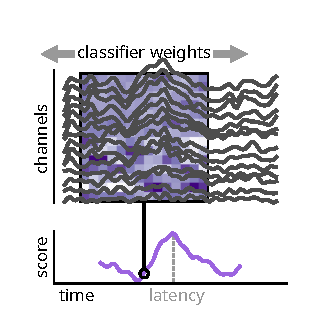
\includegraphics[width=.25\linewidth]{figures/xcorr.eps}};


				\draw[-{Latex[length=.2in]}] (epochs) to (class);
				\draw[-{Latex[length=5mm]}] (epochs) |- (class);
				\draw (class) to (xcorr);
				\draw[-{Latex[length=.2in]}] (xcorr) to (score);
				\draw (score) to (a1.center);
				\draw[-{Latex[length=5mm]}] (a1.center) -| (latency);
				\draw[-{Latex[length=5mm]}] (a1.center) -| (wav);
				\draw (epochs) |- (xcorr);
				\draw (latency) |- (a2.center);
				\draw (wav) |- (a2.center);
				\draw[-{Latex[length=5mm]}] (a2.center)  to (svm);
				\draw[color=BlockColor] (latency)  to (align);
				\draw[,color=BlockColor] (align.north)  |- (a3.center);
				\draw[-{Latex[length=5mm]},color=BlockColor] (a3.center)  to (epochs);

				\draw[color=BlockColor,dashed] (xcorr.east) to[bend left] (xcorr_fig.west);

			\end{tikzpicture}


		\end{tikzfigure}


		\subsection*{\color{black} Alignment improves SNR}
		\centering
		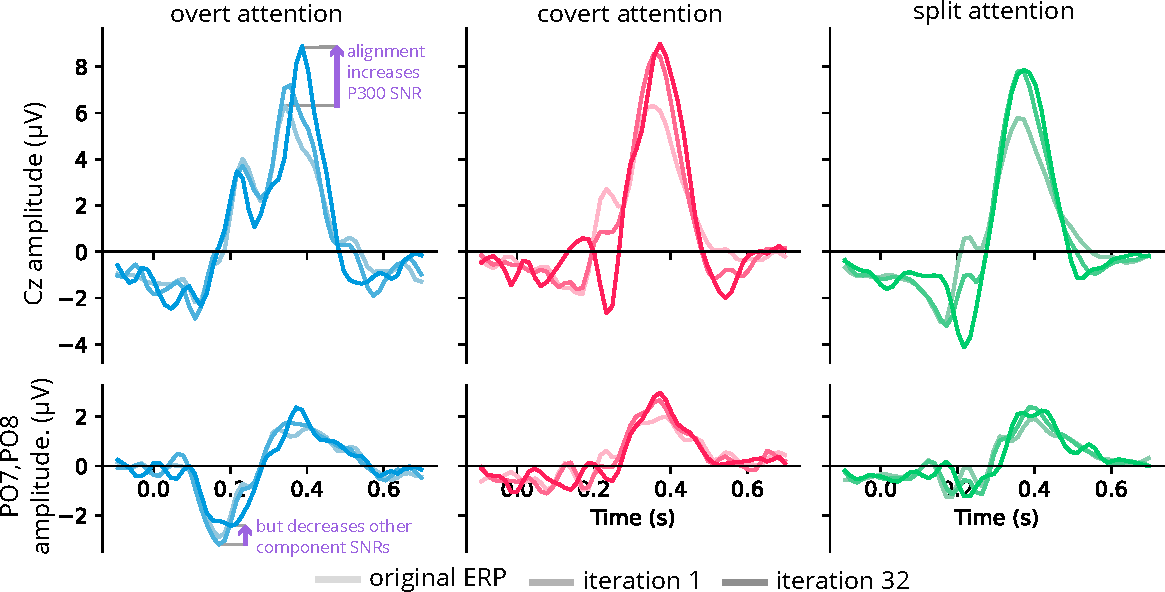
\includegraphics[width=.905\linewidth]{figures/aligned.pdf}

		\subsection*{\color{black} Convergence}
		\centering
		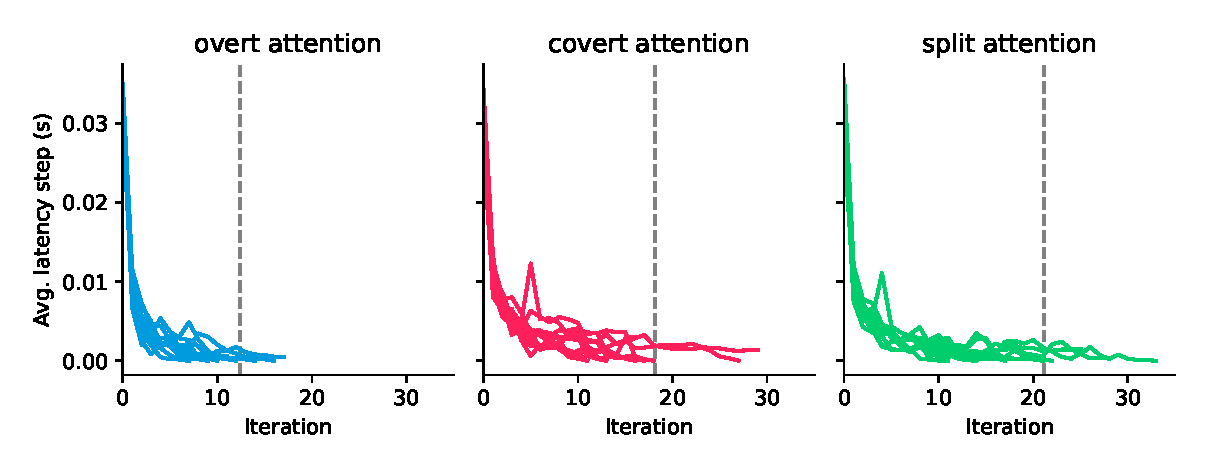
\includegraphics[width=.905\linewidth]{figures/convergence.eps}
	}

	\column{0.3333333333333333333333333333333333333333}
	\block{\circled{3} Improvement in covert attention decoding}{
		\subsection*{\color{black} Preprocessing}
		\begin{enumerate}
			\item Band-pass filter between 0.5 and 32Hz
			\item Resample to 64Hz
			\item ICA eye artifact rejection
			\item Remove bad trials according to eye-tracker
			\item Subtract non-target average
		\end{enumerate}

		\subsection*{\color{black} Single trial classification performance}

		\centering
		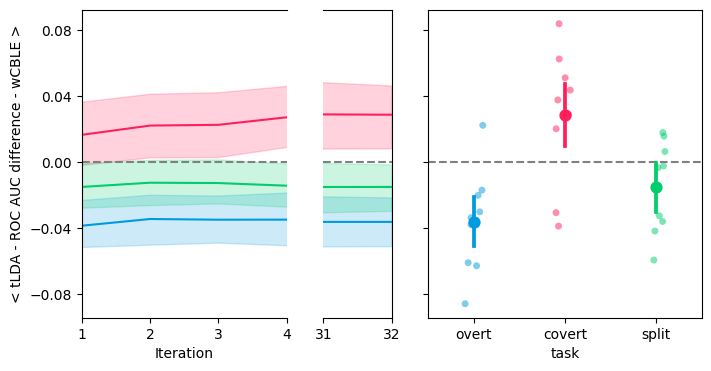
\includegraphics[width=.975\linewidth]{figures/classification_results_iter.png}

		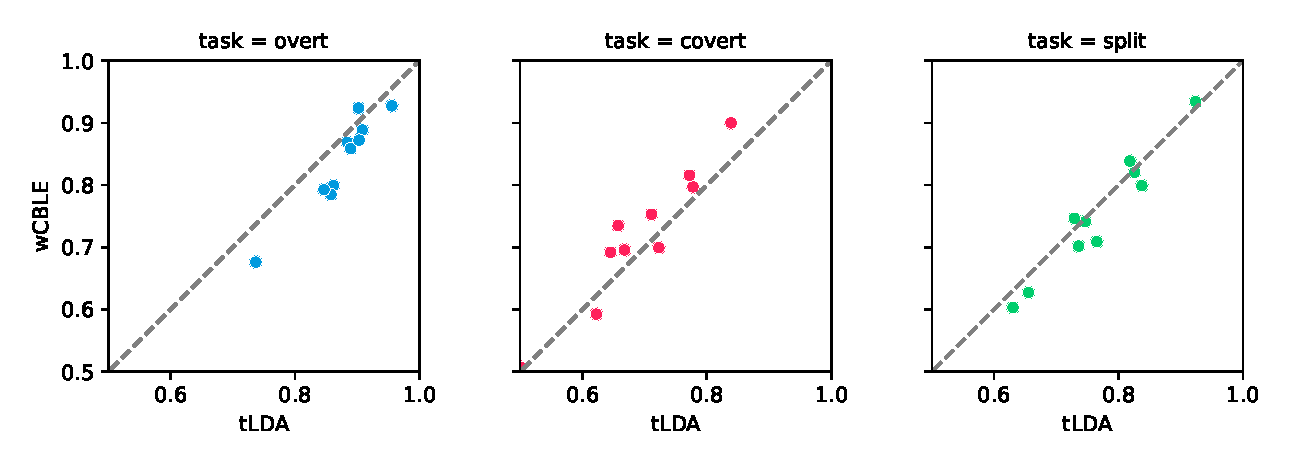
\includegraphics[width=\linewidth]{figures/classification_results_rel.eps}

		While covert attention decoding performance is significantly improved, there is a significant decrease in overt attention performance. This is probably due to the high contribution of early visual ERP components in overt attention, which are destroyed by the alignment procedure. No significant effect is observed for split attention decoding. Future work will investigate a multi-component approach.
	}

	%	\block{Conclusions}{
	%		\begin{enumerate}[label=\protect\circled{\textbf{\arabic*}}]
	%			\item Forced covert attention is not gaze-independent
	%			\item We propose a novel algorithm that can be applied in off-line and on-line decoding
	%			\item The proposed algorithm improves results in covert attention decoding, but weakens performance in the overt and the split attentoin setting.
	%		\end{enumerate}
	%	}
	\block{References} {
		\printbibliography[heading=none]
	}
\end{columns}

\end{document}
